\chapter{Démarches}
\label{ch:modele_continu}

\section{Traitement des données}
\subsection{Contexte}
Plusieurs dataset ont été utilisés pour cette étude, des données sur le descriptif des patients, sur les résultats radiomiques globaux
et multislice des patients sur leur tumeur, et enfin un jeu de données sur les observations visuelles des radiologues.
Beaucoup de données non analysables ont été retirés des dataset pour ne garder que les informations sur la forme, le niveau de gris et les textures.

\subsection{Multislicing}

L'avantage du jeu de données multislice est d'avoir des métriques sur chaque coupe de la tumeur. 
Ceci dit, la difficulté derrière est qu'un numéro de slice ne défnisse pas une région fixe du foie entre les patients
ni entre les phases d'un même patient.\\
Aussi faut-il traiter les données pour les rendre exploitables et comparables entre les patients. 
Pour ce faire, la démarche suivie est de déterminer des nouvelles métriques sur les courbes des variables en fonction
des slices (Voir Figure 2.1.)
\begin{figure}[H]
    \centering
    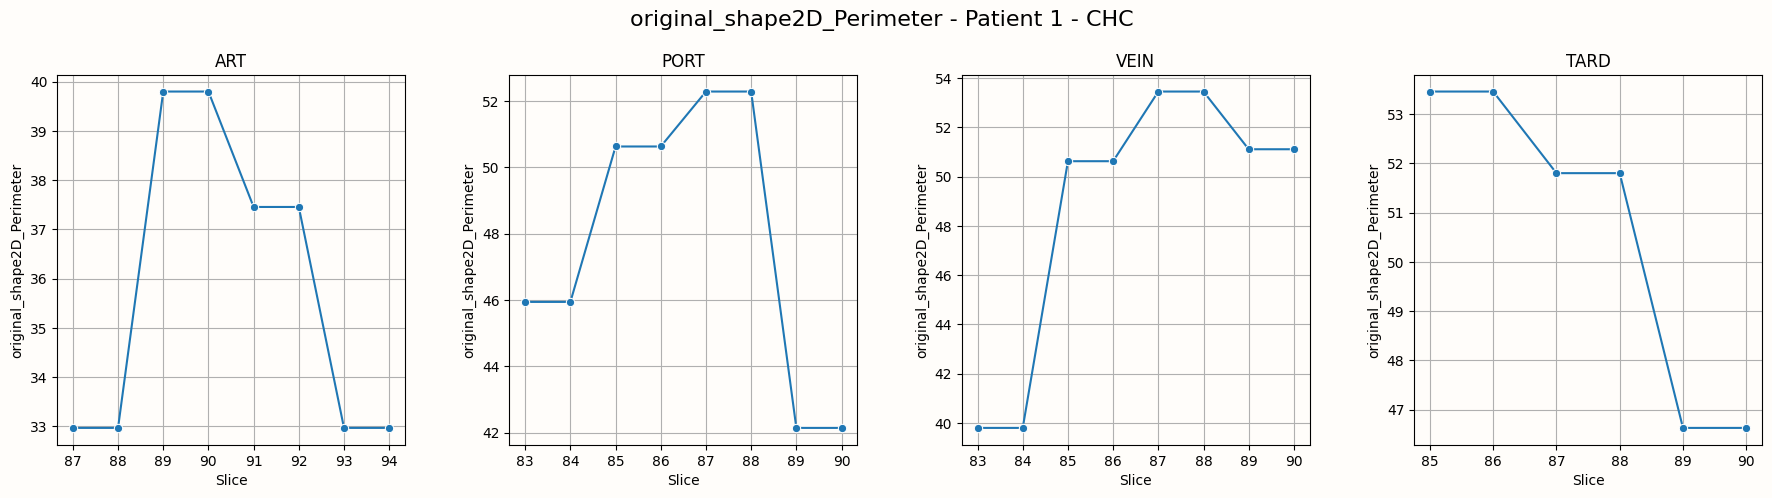
\includegraphics[width=0.5\textwidth]{img/perimeter.png}
    \caption{Courbe représentant le périmètre en fonction des slices sur les différentes phases d'un patient}
    \label{fig:perimeter}
\end{figure}

Plusieurs variables, décrivant les variations locales, ont été extraites notamment la moyenne, l'écart-type, 
la symétrie et l'énergie.

\subsection{Sélection des variables}
Une fois les données traitées, nous avons utilisé une analyse des composantes principales pour sélectionner les variables les plus 
informatives. 
